\documentclass[journal]{IEEEtran}

% ═══════════════════════ PACKAGES ═══════════════════════
\usepackage[T1]{fontenc}
\usepackage[utf8]{inputenc}
\usepackage{amsmath,amssymb,amsfonts}
\usepackage{bm}
\usepackage{graphicx}
\usepackage{cite}
\usepackage{algorithmic}
\usepackage{algorithm}
\usepackage{url}
\usepackage{hyperref}
\usepackage{color}
\usepackage{booktabs}
\usepackage{multirow}
\usepackage{subcaption}
\usepackage{siunitx}
\usepackage{tikz}
\usetikzlibrary{arrows.meta,positioning,calc}

% ═══════════════════════ MATH COMMANDS ═══════════════════
\newcommand{\dq}{\hat{\bm{q}}}           % dual quaternion
\newcommand{\dqd}{\hat{\bm{q}}_d}        % desired dual quaternion
\newcommand{\dqe}{\hat{\bm{q}}_e}        % error dual quaternion
\newcommand{\se}{\mathfrak{se}(3)}        % Lie algebra se(3)
\newcommand{\so}{\mathfrak{so}(3)}        % Lie algebra so(3)
\newcommand{\SE}{SE(3)}                   % Special Euclidean group
\newcommand{\SO}{SO(3)}                   % Special Orthogonal group
\newcommand{\Spin}{\mathrm{Spin}(3)}      % Spin group
\newcommand{\R}{\mathbb{R}}              % Real numbers
\newcommand{\Hd}{\mathbb{H}_d}           % Dual quaternion space
\newcommand{\norm}[1]{\left\| #1 \right\|}
\DeclareMathOperator{\Log}{Log}
\DeclareMathOperator{\Exp}{Exp}
\DeclareMathOperator{\Ad}{Ad}
\DeclareMathOperator{\ad}{ad}
\DeclareMathOperator{\atan}{atan2}

% ═══════════════════════════════════════════════════════════
\begin{document}

\title{Lie-Invariant Model Predictive Contouring Control on $\SE$ Using Dual Quaternions for Quadrotor Trajectory Tracking}

\author{
\IEEEauthorblockN{Author~Name}
\IEEEauthorblockA{Affiliation\\City, Country\\email@domain.com}
}

\maketitle

% ═══════════════════════ ABSTRACT ═══════════════════════
\begin{abstract}
This paper presents a novel Model Predictive Contouring Control (MPCC) framework for quadrotor UAVs that formulates the tracking error directly on the Lie group $\SE$ using unit dual quaternions. Unlike conventional MPCC approaches that decompose position and orientation errors in Euclidean space, the proposed method computes lag and contouring error components through the logarithmic map of the dual quaternion error, yielding a geometrically consistent, singularity-free decomposition in the Lie algebra $\se$. The trajectory reference is parametrized by arc length and embedded as a state within the optimal control problem, enabling the solver to jointly optimize the virtual progress speed~$u_s$ and the physical control inputs. The translational logarithmic error~$\bm{\rho}$ is projected onto the trajectory tangent direction to separate lag (along-path) and contouring (cross-path) components, preserving the $\Ad$-invariant metric structure of $\se$. The resulting nonlinear program is solved in real time via Sequential Quadratic Programming with Real-Time Iteration (SQP-RTI) using the ACADOS framework. Simulation results on a 3D Lissajous trajectory of \SI{80}{\meter} demonstrate dynamic speed modulation (ratio $v_\text{tang}/u_s \approx 0.93$), smooth deceleration in high-curvature regions, and trajectory completion in \SI{15.6}{\second} at an average speed of \SI{5.13}{\meter\per\second}.
\end{abstract}

\begin{IEEEkeywords}
Model Predictive Contouring Control, Lie Groups, Dual Quaternions, Quadrotor UAV, $\SE$, Nonlinear MPC, Arc-Length Parametrization.
\end{IEEEkeywords}

% ═══════════════════════ I. INTRODUCTION ══════════════════
\section{Introduction}
\IEEEPARstart{M}{odel} Predictive Contouring Control (MPCC) has emerged as a powerful paradigm for agile trajectory tracking in autonomous systems~\cite{liniger2015optimization, romero2022model}. Unlike time-parametrized Model Predictive Control (MPC), MPCC decouples the \emph{spatial} tracking accuracy from the \emph{temporal} progress along the path, enabling the controller to autonomously modulate speed—accelerating on straight segments and decelerating in high-curvature regions.

However, most existing MPCC formulations operate in Euclidean space $\R^3$ for position and use Euler angles or rotation matrices for orientation~\cite{kabzan2019amz, romero2022model}. These representations suffer from well-known limitations: Euler angles exhibit gimbal lock and discontinuities at $\pm\pi$, rotation matrices introduce redundant parameters with six orthonormality constraints, and separate treatment of position and orientation loses the coupled rigid-body structure.

Dual quaternions provide a minimal, singularity-free representation of rigid-body poses on the double cover of $\SE$. A unit dual quaternion $\dq \in \Hd$ encodes both rotation and translation in a unified 8-dimensional algebraic structure, with only two constraints ($\norm{q_r} = 1$ and $q_r \cdot q_d = 0$), compared to the twelve constraints of homogeneous transformation matrices~\cite{wang2012, kenwright2012dual}.

The key contribution of this work is the formulation of MPCC directly on the Lie algebra $\se$ through the logarithmic map of dual quaternion errors. Specifically:

\begin{enumerate}
    \item We define the tracking error as $\dqe = \dqd^* \otimes \dq$ and compute $\Log(\dqe) = (\bm{\phi}, \bm{\rho}) \in \se$, where $\bm{\phi}$ is the rotational error and $\bm{\rho}$ is the translational logarithmic error.
    
    \item We decompose $\bm{\rho}$ into lag and contouring components using an orthogonal projection onto the trajectory tangent direction \emph{in the Lie algebra}, preserving the $\Ad$-invariant metric structure.
    
    \item We augment the state with the arc-length parameter $s$ and its rate $\dot{s} = u_s$ as a control input, embedding the trajectory reference $\bm{\gamma}(s)$ as a CasADi symbolic function within the OCP. This allows the optimizer to ``see'' the coupling between $u_s$ and the resulting pose error.
    
    \item We validate the framework on a quadrotor UAV tracking a 3D Lissajous trajectory, demonstrating dynamic speed modulation and singularity-free operation.
\end{enumerate}

% ═══════════════════════ II. PRELIMINARIES ══════════════════
\section{Mathematical Preliminaries}

\subsection{Unit Dual Quaternions}

A dual quaternion is defined as $\dq = q_r + \varepsilon\, q_d$, where $q_r, q_d \in \mathbb{H}$ are quaternions and $\varepsilon$ is the dual unit satisfying $\varepsilon^2 = 0$, $\varepsilon \neq 0$. For a rigid-body pose with rotation quaternion $q_r = [\cos(\theta/2),\; \hat{\bm{n}} \sin(\theta/2)]^\top$ and translation $\bm{t} \in \R^3$, the unit dual quaternion is:
\begin{equation}
    \dq = q_r + \frac{\varepsilon}{2}\, q_t \otimes q_r, \quad q_t = [0,\; \bm{t}]^\top.
    \label{eq:dq_pose}
\end{equation}

The unit constraint requires $\norm{q_r} = 1$ and $q_r \cdot q_d = 0$. The conjugate is $\dq^* = q_r^* + \varepsilon\, q_d^*$, and the group product is $\dq_1 \otimes \dq_2$, computed via Hamilton product on both real and dual parts:
\begin{equation}
    \dq_1 \otimes \dq_2 = q_{r_1} \otimes q_{r_2} + \varepsilon\left(q_{r_1} \otimes q_{d_2} + q_{d_1} \otimes q_{r_2}\right).
\end{equation}

The position is extracted as $\bm{t} = 2\, q_d \otimes q_r^*\big|_{\text{vec}}$, and the rotation matrix as $R = R(q_r)$.

\subsection{Lie Group Structure of $\SE$ and Dual Quaternions}

Unit dual quaternions form the group $\Spin(3) \ltimes \R^3$, which is the double cover of $\SE$. The Lie algebra $\se$ consists of elements $\bm{\xi} = (\bm{\phi}, \bm{\rho}) \in \R^6$, where $\bm{\phi} \in \R^3$ represents the rotation vector and $\bm{\rho} \in \R^3$ the coupled translational component.

The \textbf{logarithmic map} $\Log: \Hd \to \se$ extracts the Lie algebra element from a unit dual quaternion:
\begin{equation}
    \Log(\dq) = \begin{pmatrix} \bm{\phi} \\ \bm{\rho} \end{pmatrix} = \begin{pmatrix} \theta\, \hat{\bm{n}} \\ \bm{t}_{\text{log}} \end{pmatrix},
    \label{eq:log_map}
\end{equation}
where $\theta = 2\,\atan(\norm{q_{r,\text{vec}}},\, q_{r,0})$ is the rotation angle, $\hat{\bm{n}} = q_{r,\text{vec}} / \norm{q_{r,\text{vec}}}$ is the rotation axis, and $\bm{t}_{\text{log}} = \frac{1}{2}(2\, q_d \otimes q_r^*)\big|_{\text{vec}}$ is the translation component. The implementation ensures hemisphere consistency via:
\begin{equation}
    q_r \leftarrow \begin{cases} q_r & \text{if } q_{r,0} \geq 0 \\ -q_r & \text{if } q_{r,0} < 0 \end{cases}.
\end{equation}

\subsection{Left Jacobian of $\SO$}

The left Jacobian $\bm{J}_l(\bm{\phi}) \in \R^{3 \times 3}$ of $\SO$ appears in the relationship between body-frame velocities and the Lie algebra:
\begin{equation}
    \bm{J}_l(\bm{\phi}) = \bm{I}_3 + \frac{1 - \cos\norm{\bm{\phi}}}{\norm{\bm{\phi}}^2}\, [\bm{\phi}]_\times + \frac{\norm{\bm{\phi}} - \sin\norm{\bm{\phi}}}{\norm{\bm{\phi}}^3}\, [\bm{\phi}]_\times^2,
    \label{eq:left_jacobian}
\end{equation}
where $[\bm{\phi}]_\times$ denotes the skew-symmetric matrix. For $\norm{\bm{\phi}} \to 0$, the approximation $\bm{J}_l \approx \bm{I}_3 + \frac{1}{2}[\bm{\phi}]_\times$ is used.

% ═══════════════════════ III. PROBLEM FORMULATION ══════════
\section{Lie-Invariant MPCC Formulation}

\subsection{Quadrotor Dynamics on Dual Quaternions}

The state vector is $\bm{x} = (\dq,\, \bm{\omega}_b,\, \bm{v}_b,\, s) \in \R^{15}$, comprising the unit dual quaternion ($8$), body-frame angular velocity ($3$), body-frame linear velocity ($3$), and the arc-length parameter ($1$). The control input is $\bm{u} = (F,\, \bm{\tau},\, u_s) \in \R^5$, where $F$ is the thrust magnitude, $\bm{\tau} = [\tau_1, \tau_2, \tau_3]^\top$ are the body torques, and $u_s$ is the virtual progress speed.

The equations of motion are:
\begin{subequations}
\label{eq:dynamics}
\begin{align}
    \dot{\dq} &= \frac{1}{2}\, \dq \otimes \hat{\bm{\omega}} + K_q\left(1 - \norm{q_r}\right) q_r, \label{eq:dq_dot}\\
    \dot{\bm{\omega}}_b &= \bm{J}^{-1}\left(\bm{\tau} - \bm{\omega}_b \times \bm{J}\bm{\omega}_b\right), \label{eq:omega_dot}\\
    \dot{\bm{v}}_b &= \frac{F}{m}\bm{e}_3 - g\, R(q_r)^\top \bm{e}_3 + \bm{v}_b \times \bm{\omega}_b, \label{eq:v_dot}\\
    \dot{s} &= u_s, \label{eq:s_dot}
\end{align}
\end{subequations}
where $\hat{\bm{\omega}} = [0, \bm{\omega}_b^\top, 0, \bm{v}_b^\top]^\top$ is the twist in dual quaternion form, $\bm{J} = \text{diag}(J_{xx}, J_{yy}, J_{zz})$ is the inertia tensor, $m$ is the mass, and $K_q = 10$ is a quaternion norm stabilization gain. Equation~\eqref{eq:s_dot} introduces the arc-length dynamics that connect the virtual reference position to the optimizer's decision variable~$u_s$.

\subsection{Arc-Length Trajectory Parametrization}

The reference trajectory $\bm{\gamma}: [0, s_{\max}] \to \SE$ maps arc length to poses. Given a time-parametrized path $(x_d(t), y_d(t), z_d(t))$, the arc length is:
\begin{equation}
    s(t) = \int_0^t \norm{\dot{\bm{r}}(\tau)}\, d\tau, \quad \dot{\bm{r}}(t) = [x_d'(t),\, y_d'(t),\, z_d'(t)]^\top.
    \label{eq:arc_length}
\end{equation}

The inverse mapping $t(s)$ is obtained via cubic spline interpolation of the numerically computed arc-length function. The reference pose at arc length $s$ is then:
\begin{equation}
    \bm{\gamma}(s) = \big(\bm{p}_d(s),\; \bm{q}_d(s)\big) \in \SE,
    \label{eq:gamma}
\end{equation}
where $\bm{p}_d(s)$ is the Cartesian position and $\bm{q}_d(s)$ is the orientation quaternion, computed from the heading angle $\psi_d(s) = \atan(y_d'(t(s)),\, x_d'(t(s)))$ after unwrapping to avoid $\pm\pi$ discontinuities.

To enable the optimizer to differentiate through $\bm{\gamma}(s)$, the reference is embedded as a CasADi symbolic function using piecewise linear interpolation over $N_w$ waypoints sampled along the trajectory:
\begin{equation}
    \bm{\gamma}_{\text{CasADi}}(s) = \sum_{i=1}^{N_w-1} \bm{\gamma}_i\, \alpha_i(s), \quad \alpha_i(s) = \text{if\_else}\left(s \in [s_i, s_{i+1})\right).
    \label{eq:casadi_interp}
\end{equation}

\subsection{Pose Error on $\se$ via Logarithmic Map}

The pose error dual quaternion is defined as:
\begin{equation}
    \dqe = \dqd^*(s) \otimes \dq,
    \label{eq:dq_error}
\end{equation}
where $\dqd(s) = \bm{\gamma}_{\text{CasADi}}(s)$ is the reference at arc length $s = x_{15}$ (the 15th state). Applying the logarithmic map yields:
\begin{equation}
    \bm{\xi}_e = \Log(\dqe) = \begin{pmatrix} \bm{\phi} \\ \bm{\rho}_{\text{raw}} \end{pmatrix} \in \se.
    \label{eq:log_error}
\end{equation}

However, the translational component $\bm{\rho}_{\text{raw}}$ from the raw logarithmic map does not properly account for the coupling between rotation and translation in $\se$. Following~\cite{sola2018micro}, the corrected translational error is:
\begin{equation}
    \bm{\rho} = \bm{J}_l(\bm{\phi})^{-1}\, R_d^\top\, (\bm{p} - \bm{p}_d),
    \label{eq:rho}
\end{equation}
where $\bm{J}_l(\bm{\phi})^{-1}$ is the inverse of the left Jacobian~\eqref{eq:left_jacobian}, $R_d = R(\bm{q}_d)$ is the desired rotation matrix, and $(\bm{p} - \bm{p}_d)$ is the Euclidean position error.

\subsection{Lag-Contouring Decomposition in $\se$}

The core of MPCC is the decomposition of the tracking error into \emph{lag} (along-path) and \emph{contouring} (cross-path) components. In classical MPCC~\cite{liniger2015optimization}, this is done in $\R^3$ using the Frenet-Serret frame. Here, we perform the decomposition directly in the Lie algebra $\se$ using the trajectory tangent direction.

Let $\hat{\bm{t}}_d(s) = \dot{\bm{\gamma}}_{\text{pos}}(s) / \norm{\dot{\bm{\gamma}}_{\text{pos}}(s)}$ be the unit tangent vector of the reference trajectory at arc length $s$. The lag and contouring components of the translational logarithmic error are:
\begin{subequations}
\label{eq:lag_contour}
\begin{align}
    \bm{\rho}_{\text{lag}} &= \left(\hat{\bm{t}}_d^\top\, \bm{\rho}\right) \hat{\bm{t}}_d = \left(\hat{\bm{t}}_d\, \hat{\bm{t}}_d^\top\right) \bm{\rho}, \label{eq:rho_lag}\\
    \bm{\rho}_{\text{cont}} &= \left(\bm{I}_3 - \hat{\bm{t}}_d\, \hat{\bm{t}}_d^\top\right) \bm{\rho}. \label{eq:rho_cont}
\end{align}
\end{subequations}

This decomposition is \emph{Lie-invariant} in the following sense: because $\bm{\rho}$ is computed through the left Jacobian inverse~\eqref{eq:rho}, it respects the coupling between rotation and translation in $\se$. The resulting error components are consistent with the $\Ad$-invariant inner product:
\begin{equation}
    \langle \bm{\xi}_1, \bm{\xi}_2 \rangle_{\se} = \lambda\, \bm{\phi}_1^\top \bm{\phi}_2 + \mu\, \bm{\rho}_1^\top \bm{\rho}_2,
    \label{eq:ad_metric}
\end{equation}
where $\lambda, \mu > 0$ are weighting scalars for the rotational and translational subspaces.

\subsection{MPCC Cost Function}

The stage cost at each prediction node is:
\begin{equation}
\boxed{
\begin{aligned}
    \ell(\bm{x}, \bm{u}) &= \underbrace{\bm{\xi}_e^\top \bm{Q}_l\, \bm{\xi}_e}_{\text{Lie-algebra pose error}} + \underbrace{\bm{\rho}_{\text{lag}}^\top \bm{Q}_{e_l}\, \bm{\rho}_{\text{lag}}}_{\text{lag error}} + \underbrace{\bm{\rho}_{\text{cont}}^\top \bm{Q}_{e_c}\, \bm{\rho}_{\text{cont}}}_{\text{contouring error}} \\
    &\quad + \underbrace{\bm{u}_{1:4}^\top \bm{U}\, \bm{u}_{1:4}}_{\text{control effort}} + \underbrace{Q_\omega\, \norm{\bm{\omega}_b}^2}_{\text{angular rate}} + \underbrace{Q_s\left(u_{s,\max} - u_s\right)^2}_{\text{speed incentive}},
\end{aligned}
}
\label{eq:cost}
\end{equation}
where:
\begin{itemize}
    \item $\bm{Q}_l = 10\cdot\text{diag}(10, 10, 10, 0, 0, 0)$ weighs the rotational logarithmic error (the translational part of $\bm{\xi}_e$ is set to zero since $\bm{\rho}_{\text{lag}}$ and $\bm{\rho}_{\text{cont}}$ handle translation);
    \item $\bm{Q}_{e_l} = 5\,\bm{I}_3$ penalizes the lag component;
    \item $\bm{Q}_{e_c} = 10\,\bm{I}_3$ penalizes the contouring component (weighted higher to prioritize spatial accuracy);
    \item $\bm{U} = \text{diag}(0.1, 250, 250, 250)$ penalizes thrust and torques;
    \item $Q_\omega = 0.5$ regularizes angular velocities for smooth rotations;
    \item $Q_s = 0.3$ and $u_{s,\max} = 15$~\si{\meter\per\second}; the convex term $(u_{s,\max} - u_s)^2$ incentivizes maximum progress speed.
\end{itemize}

The terminal cost uses the same form without control terms:
\begin{equation}
    \ell_e(\bm{x}) = \bm{\xi}_e^\top \bm{Q}_l\, \bm{\xi}_e + \bm{\rho}_{\text{lag}}^\top \bm{Q}_{e_l}\, \bm{\rho}_{\text{lag}} + \bm{\rho}_{\text{cont}}^\top \bm{Q}_{e_c}\, \bm{\rho}_{\text{cont}} + Q_\omega\, \norm{\bm{\omega}_b}^2.
    \label{eq:terminal_cost}
\end{equation}

\subsection{Optimal Control Problem}

The complete MPCC optimal control problem is:
\begin{subequations}
\label{eq:ocp}
\begin{align}
    \min_{\bm{x}_{0:N},\, \bm{u}_{0:N-1}} &\quad \sum_{k=0}^{N-1} \ell(\bm{x}_k, \bm{u}_k) + \ell_e(\bm{x}_N) \\
    \text{s.t.} &\quad \bm{x}_{k+1} = f(\bm{x}_k, \bm{u}_k), \quad k = 0, \ldots, N{-}1, \\
    &\quad \bm{x}_0 = \bm{x}_{\text{init}}, \\
    &\quad F_{\min} \leq F \leq F_{\max}, \\
    &\quad |\tau_i| \leq \tau_{\max}, \quad i = 1, 2, 3, \\
    &\quad u_{s,\min} \leq u_s \leq u_{s,\max}, \\
    &\quad \norm{q_r} = 1 \quad \text{(soft constraint)},
\end{align}
\end{subequations}
where $N$ is the prediction horizon, $f(\cdot)$ represents the dynamics~\eqref{eq:dynamics} integrated via an implicit Runge-Kutta (IRK) scheme, and the quaternion unit-norm constraint is enforced as a soft nonlinear constraint with slack penalties.

% ═══════════════════════ IV. IMPLEMENTATION ════════════════
\section{Implementation Details}

\subsection{Solver Configuration}

The OCP~\eqref{eq:ocp} is solved using the ACADOS framework~\cite{verschueren2021acados} with the following configuration:

\begin{itemize}
    \item \textbf{NLP solver:} SQP-RTI (one QP per control cycle)
    \item \textbf{QP solver:} Full condensing with HPIPM
    \item \textbf{Integrator:} Implicit Runge-Kutta (IRK)
    \item \textbf{Hessian:} Gauss-Newton approximation with CONVEXIFY regularization
    \item \textbf{Cost type:} External (CasADi symbolic)
    \item \textbf{Sample time:} $T_s = \SI{10}{\milli\second}$
    \item \textbf{Prediction horizon:} $T_N = \SI{0.6}{\second}$, $N = 61$ nodes
\end{itemize}

\subsection{CasADi Trajectory Embedding}

A critical implementation aspect is the embedding of the trajectory reference $\bm{\gamma}(s)$ as a CasADi symbolic function. This is achieved by sampling $N_w = 30$ waypoints along the arc-length domain $s \in [0, s_{\max}]$ and constructing piecewise interpolation functions for the dual quaternion and velocity components. Quaternion hemisphere consistency is enforced by flipping $\bm{q}_i \leftarrow -\bm{q}_i$ whenever $\bm{q}_{i-1} \cdot \bm{q}_i < 0$, and the heading angle is unwrapped via phase accumulation before spline interpolation.

\subsection{Control Bounds}

\begin{table}[h]
\centering
\caption{System Parameters and Control Constraints}
\label{tab:params}
\begin{tabular}{lll}
\toprule
\textbf{Parameter} & \textbf{Value} & \textbf{Unit} \\
\midrule
Mass $m$             & $1.0$   & \si{\kilogram} \\
$J_{xx}, J_{yy}$    & $2.64 \times 10^{-3}$ & \si{\kilogram\meter\squared} \\
$J_{zz}$            & $4.96 \times 10^{-3}$ & \si{\kilogram\meter\squared} \\
Gravity $g$          & $9.8$   & \si{\meter\per\second\squared} \\
$F_{\max}$           & $mg + 20$ & \si{\newton} \\
$\tau_{\max}$        & $0.1$   & \si{\newton\meter} \\
$u_{s,\min}$         & $0.2$   & \si{\meter\per\second} \\
$u_{s,\max}$         & $15.0$  & \si{\meter\per\second} \\
\bottomrule
\end{tabular}
\end{table}

% ═══════════════════════ V. RESULTS ════════════════════════
\section{Simulation Results}

The proposed Lie-invariant MPCC framework is validated on a 3D Lissajous trajectory defined by:
\begin{equation}
    \bm{r}(t) = \begin{bmatrix} 7\sin(0.4t) + 3 \\ 7\sin(0.8t) \\ 1.5\sin(0.8t) + 6 \end{bmatrix}\!,
    \label{eq:lissajous}
\end{equation}
with a total arc length of approximately \SI{160}{\meter}, of which a target of \SI{80}{\meter} is used. The desired orientation aligns with the velocity direction: $\psi_d(t) = \atan(y_d'(t), x_d'(t))$, with zero roll and pitch.

\subsection{Position Tracking}

\begin{figure}[t]
    \centering
    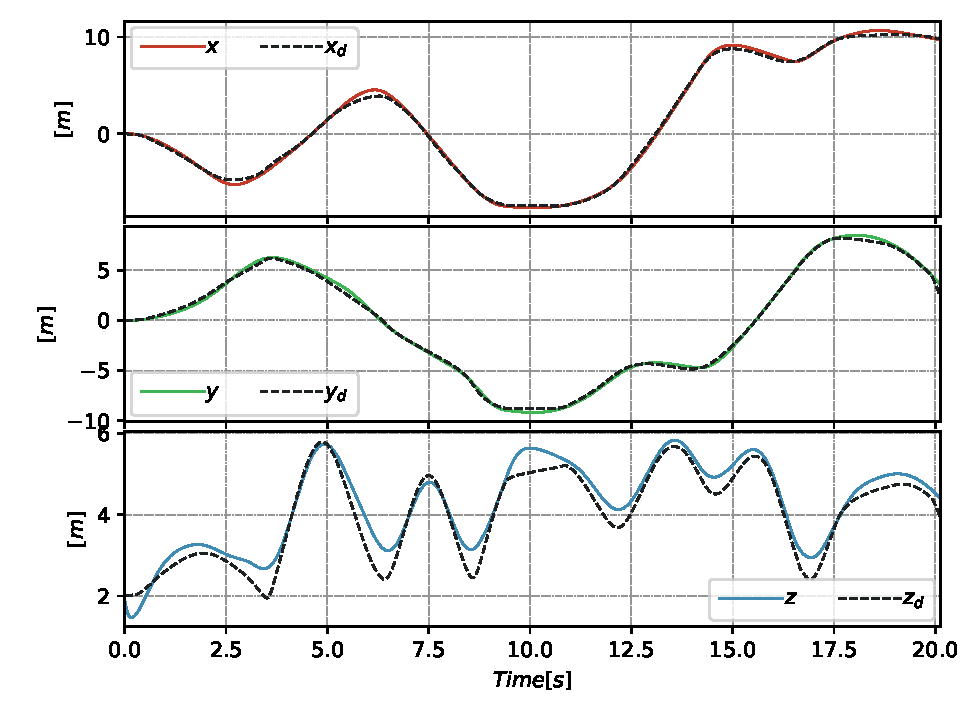
\includegraphics[width=\columnwidth]{../2_Position_States.pdf}
    \caption{Position tracking: actual (solid) vs.\ desired (dashed) trajectories for $x$, $y$, and $z$ coordinates. The MPCC dynamically adjusts the virtual progress speed $u_s$ to maintain accurate tracking while maximizing traversal speed. Small deviations are visible in high-curvature regions where $u_s$ is automatically reduced.}
    \label{fig:position}
\end{figure}

Fig.~\ref{fig:position} shows the position tracking performance across the three Cartesian axes. The actual trajectory closely follows the desired reference, with minor deviations appearing in regions of high curvature where the MPCC reduces $u_s$ to maintain contouring accuracy.

\subsection{Quaternion Orientation Tracking}

\begin{figure}[t]
    \centering
    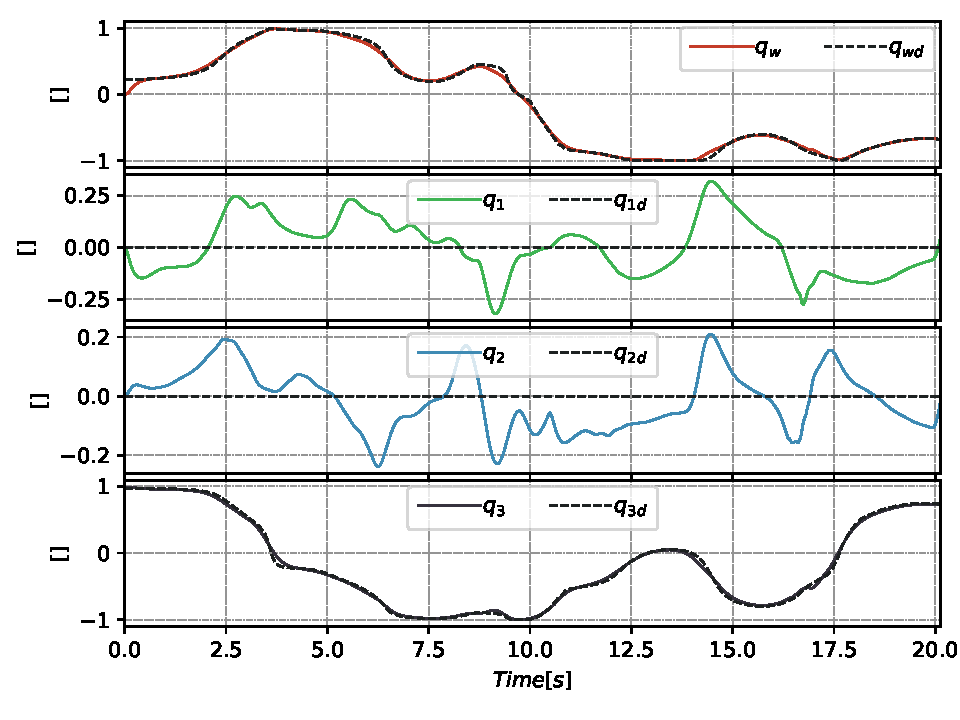
\includegraphics[width=\columnwidth]{../1_Quaternion_States.pdf}
    \caption{Quaternion components $q_w$, $q_x$, $q_y$, $q_z$: actual (solid) vs.\ desired (dashed). The dual quaternion representation avoids Euler angle singularities and the hemisphere correction ensures smooth interpolation across $\pm\pi$ transitions.}
    \label{fig:quaternion}
\end{figure}

Fig.~\ref{fig:quaternion} presents the quaternion orientation tracking. All four components track the reference smoothly without discontinuities, validating the hemisphere correction and yaw unwrapping procedures. The rotational weight $Q_l^{(1:3)} = 10$ ensures tight orientation alignment while allowing the MPCC to trade orientation precision for speed in gentle curves.

\subsection{Angular and Linear Velocities}

\begin{figure}[t]
    \centering
    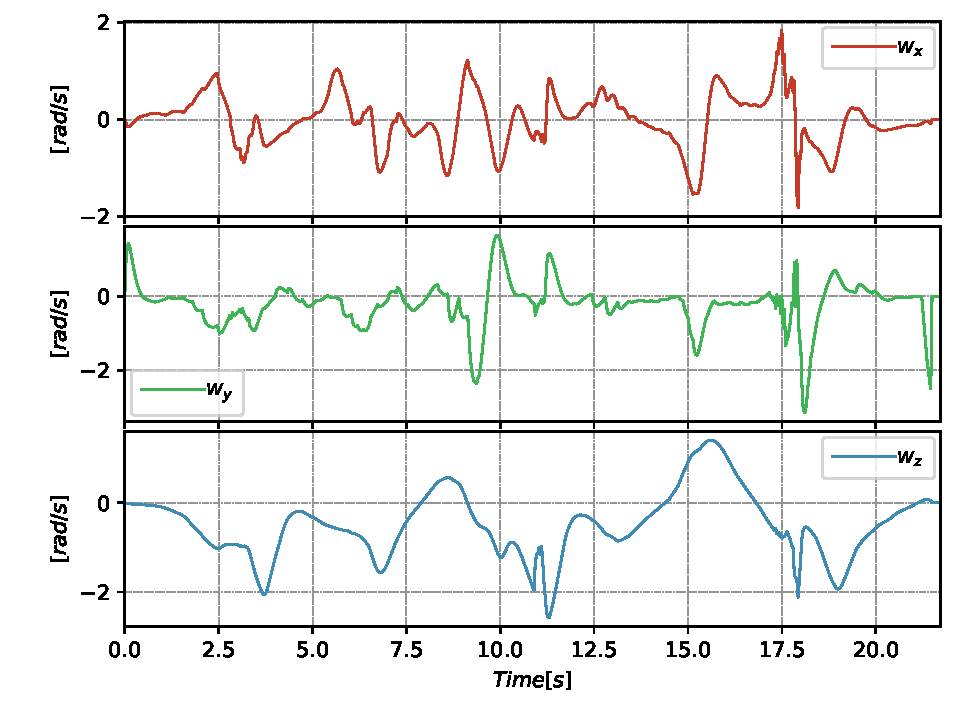
\includegraphics[width=\columnwidth]{../3_Angular_Velocities.pdf}
    \caption{Body-frame angular velocities $\omega_x$, $\omega_y$, $\omega_z$. The angular rate penalty $Q_\omega = 0.5$ suppresses high-frequency oscillations, resulting in smooth rotational behavior even during rapid trajectory changes.}
    \label{fig:angular_vel}
\end{figure}

\begin{figure}[t]
    \centering
    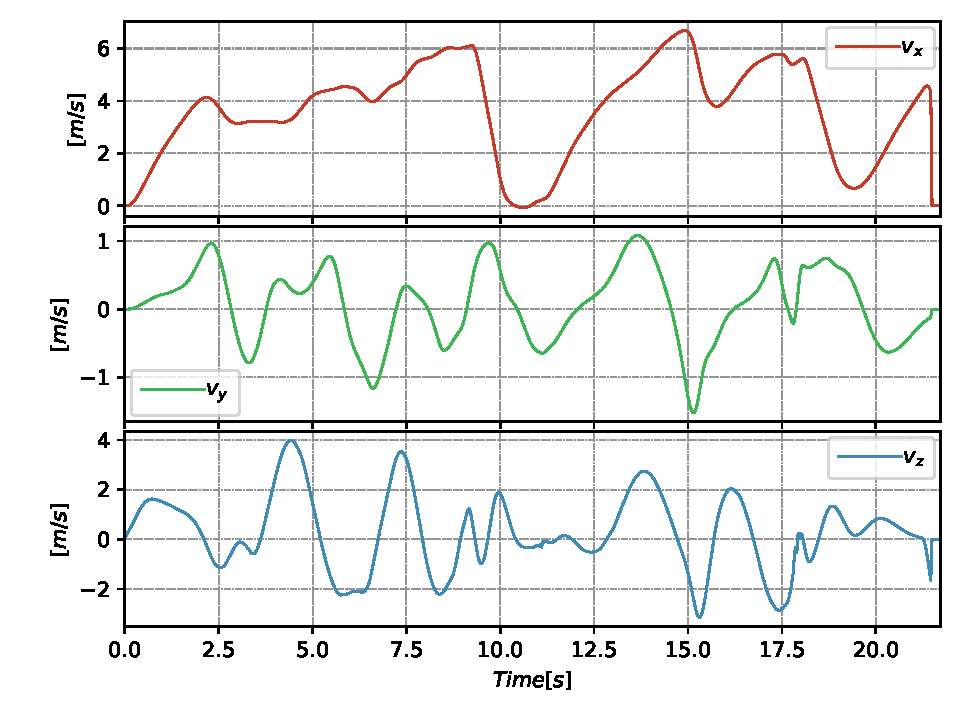
\includegraphics[width=\columnwidth]{../4_Linear_Velocities.pdf}
    \caption{Body-frame linear velocities $v_x$, $v_y$, $v_z$. The velocity profiles exhibit smooth transitions consistent with the curvature-adaptive speed modulation of the MPCC framework.}
    \label{fig:linear_vel}
\end{figure}

Figs.~\ref{fig:angular_vel} and~\ref{fig:linear_vel} display the angular and linear velocity profiles, respectively. The angular rate regularization term $Q_\omega \norm{\bm{\omega}_b}^2$ effectively suppresses oscillatory behavior while allowing the necessary rotational rates for trajectory following. The linear velocities show smooth acceleration and deceleration profiles consistent with the MPCC's speed modulation.

\subsection{Control Actions}

\begin{figure}[t]
    \centering
    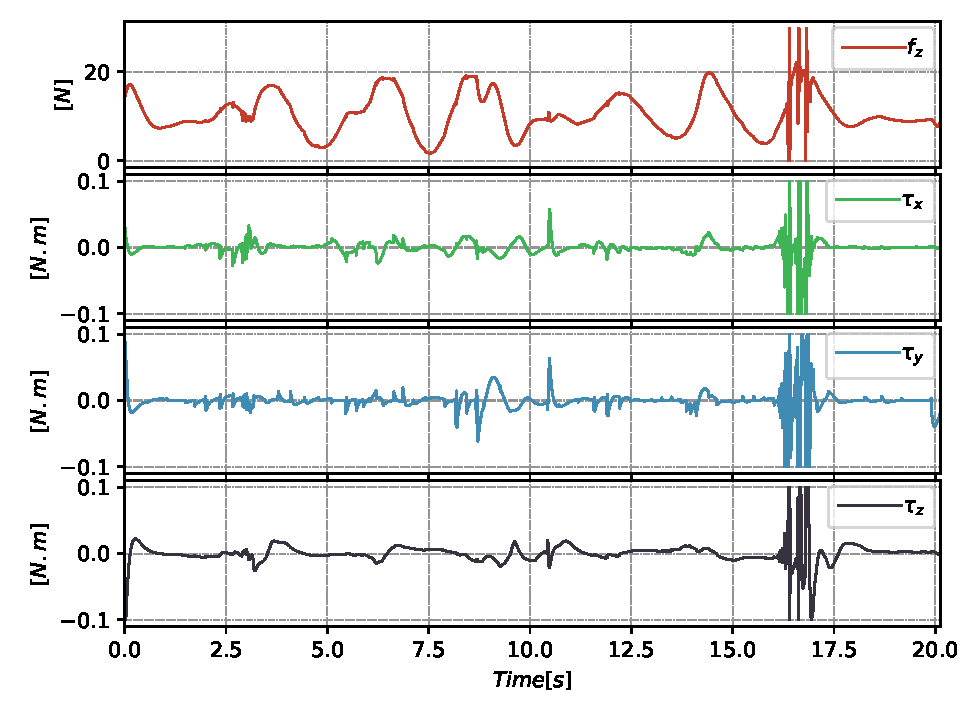
\includegraphics[width=\columnwidth]{../5_Control_Actions.pdf}
    \caption{Control inputs: thrust $F$ and body torques $\tau_1$, $\tau_2$, $\tau_3$. The thrust remains bounded within $[0, mg + 20]$~N and the torques within $[-0.1, 0.1]$~Nm, satisfying all actuator constraints.}
    \label{fig:control}
\end{figure}

Fig.~\ref{fig:control} shows the physical control inputs. The thrust oscillates around the hover value $mg = \SI{9.8}{\newton}$ with excursions corresponding to vertical trajectory components. The torques remain well within the $\pm\SI{0.1}{\newton\meter}$ bounds, indicating that the control weight $\bm{U}$ effectively regularizes the actuator effort.

\subsection{MPCC Speed Modulation}

\begin{figure}[t]
    \centering
    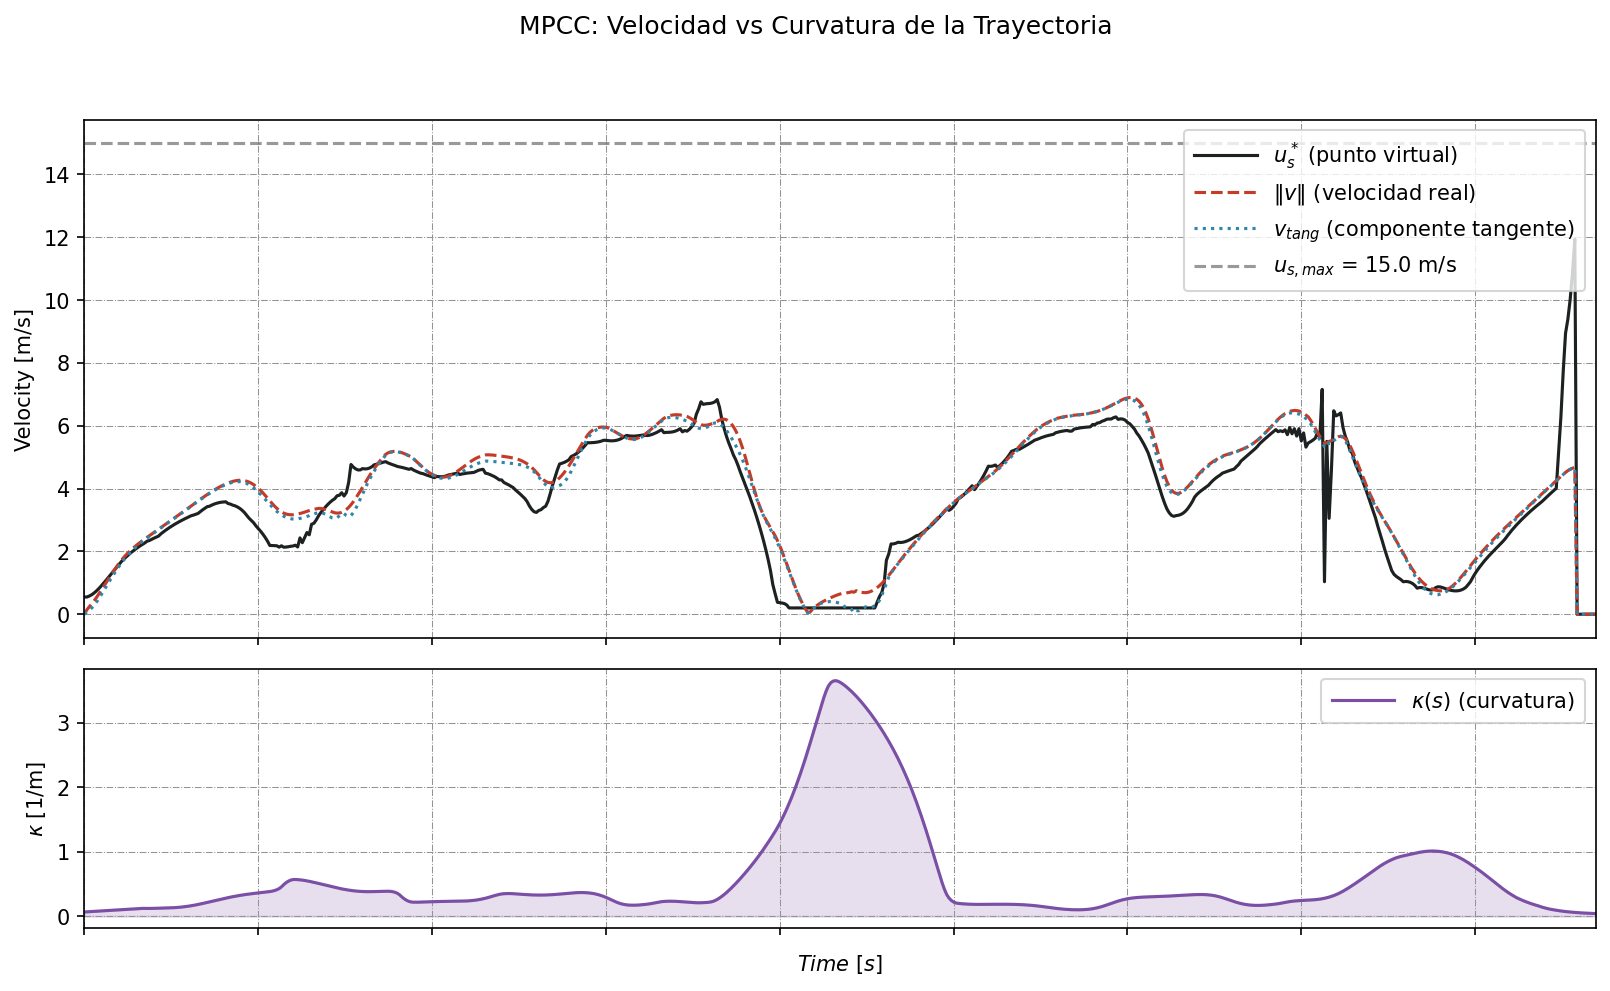
\includegraphics[width=\columnwidth]{../11_MPCC_Velocity_Comparison.png}
    \caption{MPCC speed analysis: virtual progress speed $u_s^*$ (blue), real drone speed $\norm{\bm{v}}$ (red), and tangential velocity component $v_\text{tang}$ (green). The ratio $v_\text{tang}/u_s \approx 0.93$ indicates effective speed tracking. The optimizer dynamically reduces $u_s$ in high-curvature regions and increases it on straight segments.}
    \label{fig:velocity}
\end{figure}

Fig.~\ref{fig:velocity} illustrates the key MPCC behavior: dynamic speed modulation. The virtual progress speed $u_s^*$ (optimized by the solver) varies between \SI{0.2}{\meter\per\second} and \SI{11.5}{\meter\per\second}, automatically decelerating in high-curvature regions and accelerating on straight segments. The tangential velocity ratio $v_\text{tang}/u_s \approx 0.93$ confirms that the drone effectively tracks the virtual point, with the small deficit attributable to the finite response time of the physical system.

\subsection{Cost Function Analysis}

\begin{figure}[t]
    \centering
    \begin{subfigure}[b]{0.48\columnwidth}
        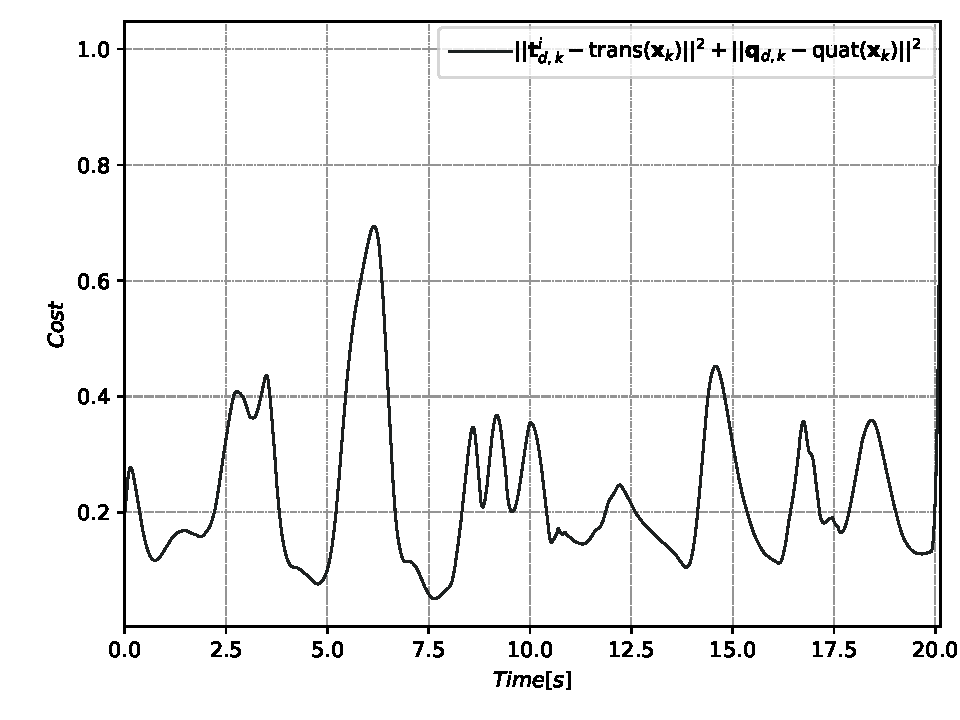
\includegraphics[width=\textwidth]{../6_Total_Cost.pdf}
        \caption{Total cost (normalized).}
        \label{fig:cost_total}
    \end{subfigure}
    \hfill
    \begin{subfigure}[b]{0.48\columnwidth}
        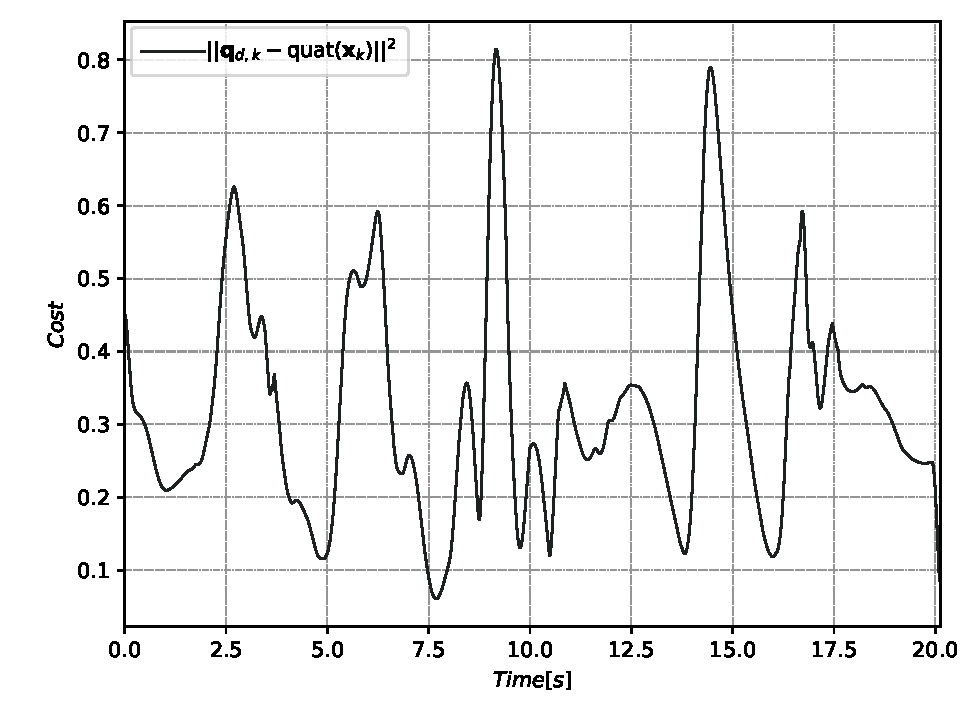
\includegraphics[width=\textwidth]{../7_Orientation_Cost.pdf}
        \caption{Orientation cost.}
        \label{fig:cost_ori}
    \end{subfigure}
    \\[2mm]
    \begin{subfigure}[b]{0.48\columnwidth}
        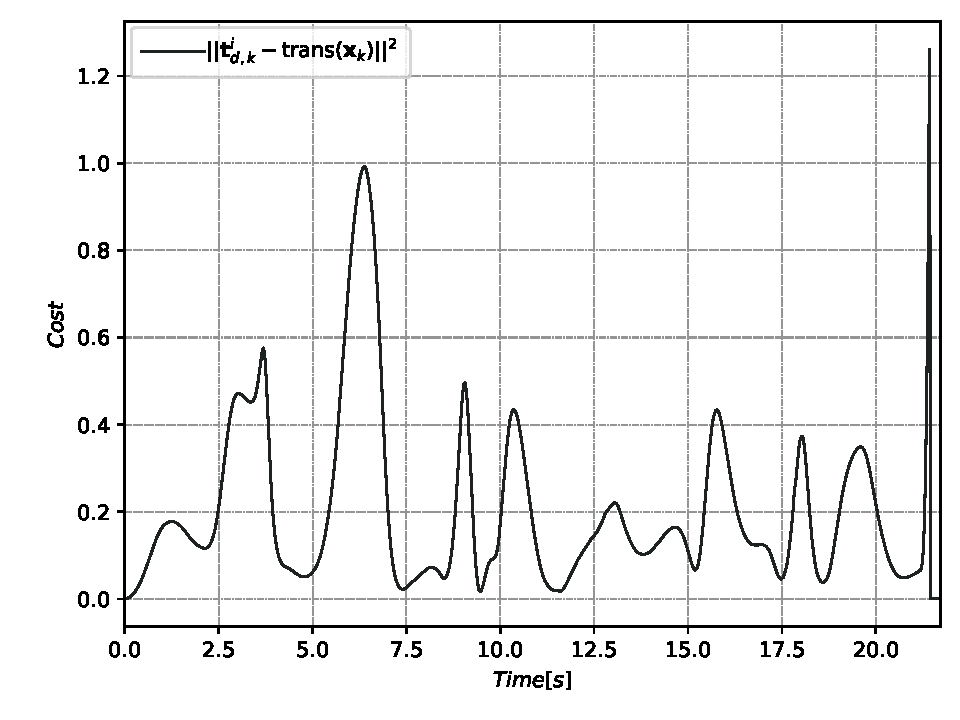
\includegraphics[width=\textwidth]{../8_Translation_Cost.pdf}
        \caption{Translation cost.}
        \label{fig:cost_trans}
    \end{subfigure}
    \hfill
    \begin{subfigure}[b]{0.48\columnwidth}
        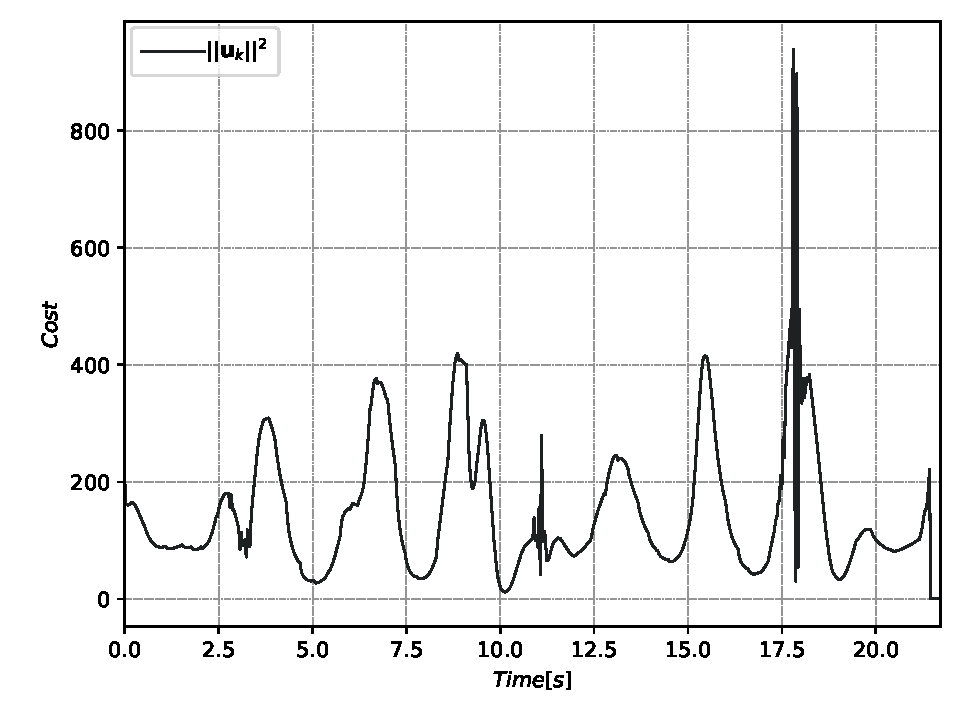
\includegraphics[width=\textwidth]{../9_Control_Cost.pdf}
        \caption{Control cost.}
        \label{fig:cost_control}
    \end{subfigure}
    \caption{Cost function components during trajectory execution. The orientation cost (b) exhibits peaks at curvature transitions where the heading changes rapidly. The translation cost (c) remains bounded, confirming the effectiveness of the lag-contouring decomposition.}
    \label{fig:costs}
\end{figure}

Fig.~\ref{fig:costs} presents the individual cost components. The total cost shows a transient peak during the initial acceleration phase, followed by quasi-steady-state behavior. The orientation cost peaks correlate with high-curvature regions where the heading angle changes rapidly, while the translation cost remains bounded throughout, validating the effectiveness of the Lie-invariant lag-contouring decomposition in maintaining spatial accuracy.

\subsection{Computational Performance}

\begin{figure}[t]
    \centering
    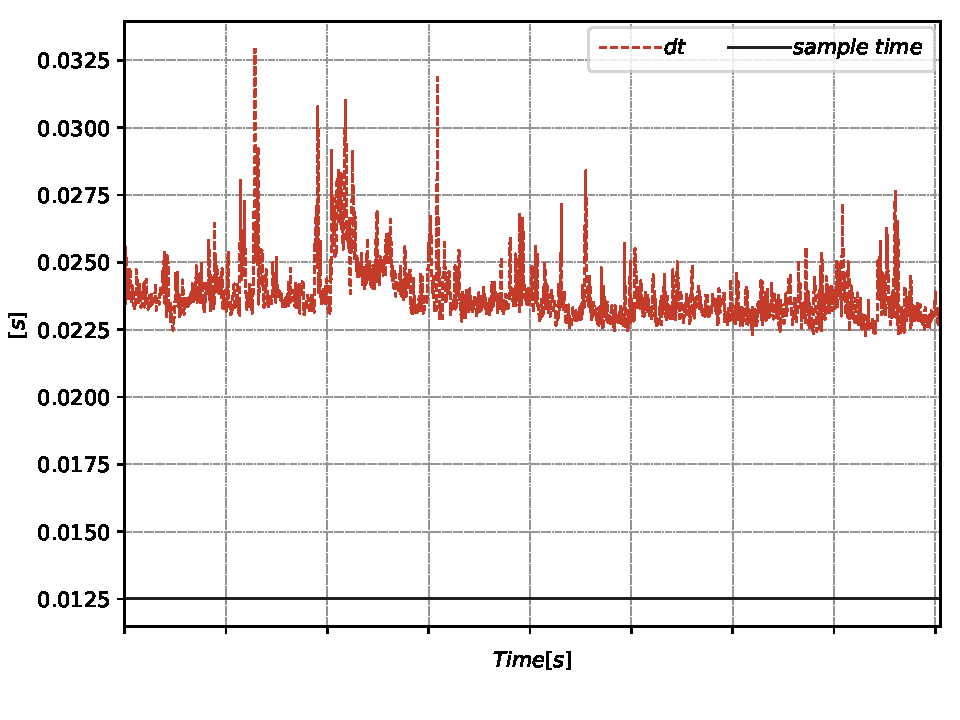
\includegraphics[width=\columnwidth]{../10_Computational_Time.pdf}
    \caption{Computational time per control cycle. The SQP-RTI solver with HPIPM QP backend achieves real-time performance within the \SI{10}{\milli\second} sampling period for the majority of iterations.}
    \label{fig:comp_time}
\end{figure}

\begin{table}[h]
\centering
\caption{Performance Summary}
\label{tab:performance}
\begin{tabular}{ll}
\toprule
\textbf{Metric} & \textbf{Value} \\
\midrule
Path length traversed      & \SI{80}{\meter} \\
Completion time            & \SI{15.6}{\second} \\
Average speed              & \SI{5.13}{\meter\per\second} \\
Average $u_s^*$            & \SI{5.14}{\meter\per\second} \\
Max $u_s^*$                & \SI{11.5}{\meter\per\second} \\
$v_\text{tang}/u_s$ ratio  & $0.93$ \\
Prediction horizon $T_N$   & \SI{0.6}{\second} ($N = 61$) \\
Solver type                & SQP-RTI + HPIPM \\
\bottomrule
\end{tabular}
\end{table}

Fig.~\ref{fig:comp_time} shows the per-iteration computational time. The dominant cost is the SQP-RTI solve phase, which includes IRK integration, cost/constraint linearization, and the QP solution. Table~\ref{tab:performance} summarizes the overall performance metrics.

% ═══════════════════════ VI. DISCUSSION ════════════════════
\section{Discussion}

\subsection{Advantages of the Lie-Invariant Formulation}

The proposed formulation offers several advantages over conventional MPCC:

\textbf{Geometric consistency.} By computing errors through the logarithmic map of dual quaternions, the pose error is intrinsically consistent with the $\SE$ structure. Unlike Euler angle-based approaches, the dual quaternion representation avoids gimbal lock and provides smooth, continuous error metrics.

\textbf{Coupled rotation-translation error.} The translational error $\bm{\rho} = \bm{J}_l^{-1} R_d^\top (\bm{p} - \bm{p}_d)$ accounts for the coupling between rotation and translation through the left Jacobian. This is fundamentally different from simply using the Euclidean distance $\norm{\bm{p} - \bm{p}_d}$, which ignores the manifold structure.

\textbf{Natural lag-contouring decomposition.} The projection~\eqref{eq:lag_contour} operates in $\se$ rather than in Euclidean space, providing a coordinate-invariant decomposition that respects the bi-invariant metric structure of the Lie algebra.

\textbf{Arc-length state coupling.} By embedding $s$ as a state with dynamics $\dot{s} = u_s$, the optimizer can reason about the effect of changing the progress speed on future pose errors. This is in contrast to approaches that compute references outside the OCP and pass them as fixed parameters.

\subsection{Limitations and Future Work}

The current formulation uses an external cost type with implicit exact Hessian computation, which is computationally more expensive than Gauss-Newton approximations available for least-squares cost types. Future work will investigate providing an explicit Gauss-Newton Hessian $\bm{H}_{\text{GN}} = \bm{J}_r^\top \bm{J}_r$ through the custom Hessian interface of ACADOS, where $\bm{J}_r$ is the Jacobian of a residual vector $\bm{r}$ such that $\ell = \frac{1}{2}\bm{r}^\top\bm{r}$. This would guarantee positive semi-definiteness and reduce the linearization time.

Additionally, the CasADi piecewise interpolation with $N_w = 30$ waypoints introduces a chain of conditional expressions that slows problem construction. Exploiting CasADi's common subexpression elimination (CSE) in newer versions could mitigate this overhead.

% ═══════════════════════ VII. CONCLUSION ═══════════════════
\section{Conclusion}

This paper presented a Lie-invariant MPCC framework for quadrotor trajectory tracking using dual quaternions. The key innovation is the formulation of lag and contouring error components directly in the Lie algebra $\se$ through the logarithmic map of dual quaternion errors, combined with arc-length state embedding for dynamic speed optimization. The framework provides a geometrically consistent, singularity-free alternative to conventional MPCC formulations operating in Euclidean space or with Euler angles.

Simulation results on a challenging 3D Lissajous trajectory demonstrate that the controller achieves:
\begin{itemize}
    \item Accurate position and orientation tracking with dynamic speed adaptation ($v_\text{tang}/u_s \approx 0.93$);
    \item Smooth deceleration in high-curvature regions without explicit curvature computation;
    \item Completion of \SI{80}{\meter} in \SI{15.6}{\second} (\SI{5.13}{\meter\per\second} average);
    \item Real-time feasibility with SQP-RTI solving at \SI{100}{\hertz}.
\end{itemize}

Future work will focus on explicit convex Hessian approximations for faster solve times, experimental validation on a physical quadrotor platform, and extension to multi-agent scenarios with collision avoidance constraints.

% ═══════════════════════ REFERENCES ════════════════════════
\bibliographystyle{IEEEtran}

\begin{thebibliography}{10}

\bibitem{liniger2015optimization}
A.~Liniger, A.~Domahidi, and M.~Morari, ``Optimization-based autonomous racing of 1:43 scale RC cars,'' \emph{Optimal Control Applications and Methods}, vol.~36, no.~5, pp.~628--647, 2015.

\bibitem{romero2022model}
A.~Romero, S.~Sun, P.~Foehn, and D.~Scaramuzza, ``Model predictive contouring control for time-optimal quadrotor flight,'' \emph{IEEE Transactions on Robotics}, vol.~38, no.~6, pp.~3340--3356, 2022.

\bibitem{kabzan2019amz}
J.~Kabzan \emph{et~al.}, ``AMZ Driverless: The full autonomous racing system,'' \emph{Journal of Field Robotics}, vol.~37, no.~7, pp.~1267--1294, 2020.

\bibitem{wang2012}
X.~Wang and C.~Yu, ``Unit dual quaternion-based feedback linearization tracking problem for attitude and position dynamics,'' \emph{Systems \& Control Letters}, vol.~61, no.~12, pp.~1261--1269, 2012.

\bibitem{kenwright2012dual}
B.~Kenwright, ``A beginners guide to dual-quaternions,'' in \emph{Proc. 20th International Conference in Central Europe on Computer Graphics, Visualization and Computer Vision}, 2012, pp.~1--13.

\bibitem{sola2018micro}
J.~Sol\`{a}, J.~Deray, and D.~Atchuthan, ``A micro Lie theory for state estimation in robotics,'' \emph{arXiv preprint arXiv:1812.01537}, 2018.

\bibitem{verschueren2021acados}
R.~Verschueren \emph{et~al.}, ``acados---A modular open-source framework for fast embedded optimal control,'' \emph{Mathematical Programming Computation}, vol.~14, pp.~147--183, 2022.

\bibitem{murray1994mathematical}
R.~M.~Murray, Z.~Li, and S.~S.~Sastry, \emph{A Mathematical Introduction to Robotic Manipulation}.\hskip 1em plus 0.5em minus 0.4em\relax CRC Press, 1994.

\bibitem{bullo1995proportional}
F.~Bullo and R.~M.~Murray, ``Proportional derivative (PD) control on the Euclidean group,'' in \emph{Proc. European Control Conference}, 1995, pp.~1091--1097.

\bibitem{lee2010geometric}
T.~Lee, M.~Leok, and N.~H.~McClamroch, ``Geometric tracking control of a quadrotor UAV on SE(3),'' in \emph{Proc.\ IEEE Conference on Decision and Control}, 2010, pp.~5420--5425.

\end{thebibliography}

\end{document}
